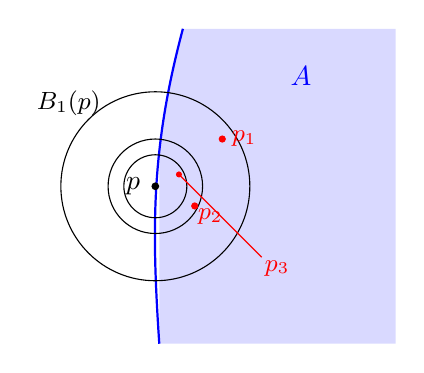
\begin{tikzpicture}
  \begin{scope}
    \clip (0,-2) rectangle (3,2);
    \fill[blue, opacity=0.15] (0,-2) .. controls (-0.1,-0.5) and (-0.1,0.5) .. (0.3,2) -- (3,2) -- (3,-2) -- cycle;
  \end{scope}
  \draw[blue, thick] (0,-2) .. controls (-0.1,-0.5) and (-0.1,0.5) .. (0.3,2);
  \node[blue] at (1.8,1.4) {$A$};
  \coordinate (p) at (-0.05,0);
  \fill (p) circle (1.4pt) node[left, xshift=-2pt] {$p$};
  \draw (p) circle (1.2);
  \draw (p) circle (0.6);
  \draw (p) circle (0.4);
  \node at (-1.15,1.05) {\small $B_1(p)$};
  \fill[red] (0.8,0.6) circle (1.3pt) node[right] {\small $p_1$};
  \fill[red] (0.45,-0.25) circle (1.3pt) node[below right, inner sep=1pt] {\small $p_2$};
  \fill[red] (0.25,0.15) circle (1.1pt);
  \draw[red] (0.25,0.15) -- (1.3,-0.9) node[below right, inner sep=1pt] {\small $p_3$};
\end{tikzpicture}
